\section {Introduction (and Inspiration/Motivation)}
%\textbf{}
In this study, non-institutional yet societally-determined antonyms for nouns —specifically, non-modified nouns—are shown to exist.  Since nouns such as $male$ \opp $female$, $feminine$ \opp $masculine$, $boy$ \opp $girl$ are generally accepted to be pairs of opposites, the term non-modified noun will be used to refer to non-gender nouns or nouns that are not modified by an adjective (e.g. red carpet).  Meanwhile, the term noun will be used in the general sense to refer to any noun, including abstract nouns.  The tilde, \oppnospace, will be used to denote an antonym pairing such as $hot$ \opp $cold$.  

A discussion will follow concerning the possibility that abstracted application of the rules that govern institutionalized opposites is what govern the majority (if not all) of antonyms for unmodified nouns.  In other words, this study takes the step to determine whether rules for generation of standard antonyms can be applied more generally to even the most concrete of nouns, rules which must act in tak-like manner in order to apply more generally than they normally would.

\subsection {Antonym Usage: Paradox and Middle-ground} Only two usages of antonyms will be touched on here, paradox and middle ground.  For a discussion on other usages such as implicit and explicit comparison, \citeA<see>{Zhang}.  

Citing a Latin example \textit{neque vivus neque mortuus} (not alive not dead), Bertocchi notes that antonyms can be used to create a paradox (Bertocchi 2003).  This usage is not in question.  However, this same construction is not paradoxical in all cases.  Take for example the case of $heavy$ \opp $light$, forming the phrase \textit{not heavy not light}.  This is simply another way to express \textit{medium}.  In some given language a term for medium may not exist and whether it is paradoxical or not is up to the native speakers of the language.  Meanwhile, languages which have a form to describe medium would say it is simply a middle ground and not a paradox. 

Assuming that antonyms exist for non-modified nouns, middle ground usages exist as well.  Take the following example: I want a pencil-pen---something that looks like a pen, but that is still erasable.  In this case, the middle-ground might exist, but the speaker does not choose to select something which would fit the criteria, perhaps because they do not know that erasable pens exist.  The speaker uses opposition, two extremes, to create an enclosure automatically defining the possible characteristics (or non-characteristics) that are inherent in the desire.  In this case, the speaker highlights key characteristics by saying ``something that looks like a pen, but that is still erasable.''

\subsection {Classification: Gradable vs. Non-gradable} For institutionally-accepted antonyms, two main types of antonyms exist: gradable and non-gradable. Bertocchi calls gradable antonyms contraries, while non-gradable antonyms are contradictories.   Non-gradables, or contradictories are binary, but also have no middle ground (Bertocchi 2003).  A good example of a set of contradictories could be $boy$ \opp $girl$.  There is no in-between state possible for something which could be one or the other.  As for contraries, the middle ground does exist.  A good example of this is $large$ \opp $small$, the middle ground, of course, being medium.  

This study will reveal the existence of a greater number of categories for concrete antonyms than for abstract nouns. 

\subsection {Attributes of Traditional Antonymy} Besides the ability to be classified as either gradable or non-gradable, antonyms tend to binary, communicative, and transitive.  Unfortunately, corollary attributes for concrete antonyms cannot be proven by this study; this study was created to establish the existence of concrete antonyms.

\subsection {Dichotomy} Traditional opposites tend to be binary or dichotomous.  Lindner states ``The opposition relation is built squarely on a dichotomy or binary contrast of some sort.'' (Lindner 1982) In such cases, one term can be understood by using the negated form of its opposite.  This works only when considering optimal pairing partners for a given adjective.  Take for example \textit{small}.  Both \textit{big} and \textit{large} could be accepted as opposites, but depending on the circumstance, \textit{big} or \textit{large} is the optimal partner.

\subsection {Communicativity} To be communicative, given one adjective $X$ whose best opposite is $Y$, $Y$’s best opposite must be $X$.  This is easily the case for traditional antonyms as they tend to be contained in obviously binary sets. In mathematical notation, where  denotes two-way implication, this would be: $X$ \opp $Y$, $Y$ \opp $X$.

\subsection {Transitivity} For adjectives (and perhaps other abstract parts of speech), one can find the antonym for word $X$ by finding an antonym, $Y$, for one of $X$’s synonyms, $Z$.  This is a transitive process.  In a mathematical notation where = denotes synonymy, this would be: $X = Z$, $Z$ \opp $Y$ => $X$ \opp $Y$.

\subsection {Institutional Paradox} In English, there words for which antonyms are well-known and, indeed, institutionalized.  These include adjectives, adverbs, and some abstract nouns.  The more abstract parts of speech can have their corollary synonyms and antonyms while more concrete parts of speech only have synonyms (nouns). This presents a well-accepted paradox; abstract terms can undergo a process or rule to generate an institutionalized opposite, but the underlying rule that functions so easily upon abstract parts of speech does not work as prevalently on more concrete parts of speech!  Figure ~\ref{fig:introFig} visualizes this paradox.

Gender nouns and modified nouns are marked in red in Figure ~\ref{fig:introFig} because they act differently than normal nouns; they can and often have institutionalized antonyms in spite of the fact that they are concrete.  For adjectivally-modified nouns, this must be due to the presence of the adjectives which enable the nouns to become highly institutionalized as well.  Gender nouns act as if they are adjectivally-modified nouns, perhaps because they are modified internally (charged with gender).  Since adjectives tend to be binary (when an opposite exists), the modified and gender nouns are polarized, meaning that they are to be paired with an antonym in spite of their concreteness.  Examples pairs include: $female$ \opp $male$, $man$ \opp $woman$, $negative~electron$ \opp $positive~electron$, $hen$ \opp $tom$, $boy$ \opp $girl$.  Note that some of these nouns can be used as adjectives ($female$ \opp $male$, $novice$ \opp $expert$), and perhaps that is where their dichotomy was born.  Such pairings are binary---an attribute typical of adjectives as far as antonyms are concerned.  Gender nouns and modified nouns are indeed exceptional.  Whether they are more concrete than abstract is up for question.  Figure ~\ref{fig:introFig} treats them as highly concrete.  Perhaps they are both.    

\begin{figure}[here]
	\centering
	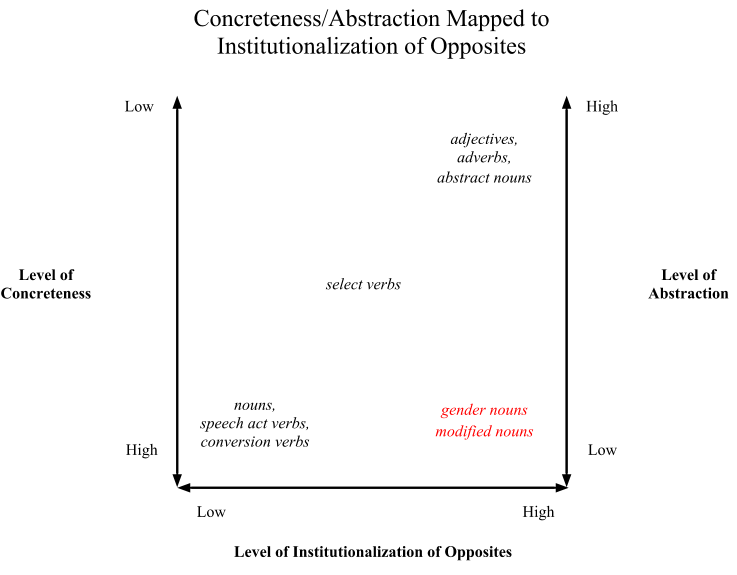
\includegraphics[width=0.9\textwidth]{images/Diagram.png}
	\caption{Concreteness/Abstraction mapped to institutionalization of opposites.  Red is used to demarcate word types which are marked.}
	\label{fig:introFig}
\end{figure}
	
Note also that abstract nouns are listed separately from adjectives and adverbs; although they are classified as nouns, they are actually very abstract.  They are nouns because they can be treated as subjects in a sentence and can receive many of the same theta roles that concrete nouns receive.  
Antonyms for abstract nouns are highly institutionalized just as those for adjectives are.  Examples include: belief \opp disbelief; $faith$ \opp $skepticism$; $love$ \opp $hatred$; $hope$ \opp $discouragement$, $hopelessness$; $unity$ \opp $disunity$, $partiality$.

\subsection {Adjective vs. Nouns Vs. Adjectivally-Modified Nouns}  Traditionally, adjectives can have both antonyms and synonyms, while non-modified nouns can have only synonyms.  This would make it difficult to define a concrete noun based on its opposite—unless it is modified.  Thus, to describe a house in terms of its opposite is traditionally impossible, unless it is described as being tall, in which case part of its definition could describe it as not short.  So, when concrete nouns are modified, a portion of their definition may include its antonym.  This is a contrived example, but one might imagine a more complex adjective modification that lends itself more towards definition via description in terms of opposites than by traditional means of definition.  

\subsection {Opposition in Semantic Primitives} Semantic primitives make up the core meaning of language (Wierzbicka 2009).  Wierzbicka says that semantic primitives are only definable in terms of themselves.  However, in her list of semantic primitives she includes a negating mechanism, NOT (Wierzbicka 2009).  It is this very mechanism which leads one to believe that opposition exists at the root of the meaning of language and since it exists in her list of semantic primitives, one must believe that negation of semantic primitives, including the negation/opposition of nouns (especially given such a small list) is not outside the realm of possibilities for the human mind. 

%\section {Side A.} 

\section {Side B.} 

